\documentclass{article}
\usepackage{CJKutf8}
\usepackage[utf8]{inputenc}
\usepackage[left=2.50cm, right=2.50cm, top=2.50cm, bottom=2.50cm]{geometry}
\usepackage[unicode=true,colorlinks,urlcolor=blue,linkcolor=blue,bookmarksnumbered=true]{hyperref}
\usepackage{latexsym,amssymb,amsmath,amsbsy,amsopn,amstext,amsthm,amsxtra,color,bm,calc,ifpdf}
\usepackage{enumerate}
\usepackage{fancyhdr}
\usepackage{listings}
\usepackage{multirow}
\usepackage{makeidx}
\usepackage{subfigure}
\usepackage{graphicx}
\begin{document}
\begin{CJK}{UTF8}{gbsn}
\section{Pytorch}
1、
\section{第2章标题}

以下是一些样例:

\textbf{加粗文本}

\textit{倾斜文本}

\underline{下划线文本}

项目编号:

\begin{itemize}
    \item XXX
    \item XXX
    \item XXX
\end{itemize}

\begin{enumerate}
    \item XXX
    \item XXX
    \item XXX
\end{enumerate}

行内公式:$\int_a^b f(x)dx = F(b)-F(a)$

另起一行的公式:中建
\begin{equation}
    \int_a^b f(x)dx = F(b)-F(a)
\end{equation}
\begin{figure}[h]
	\centering
	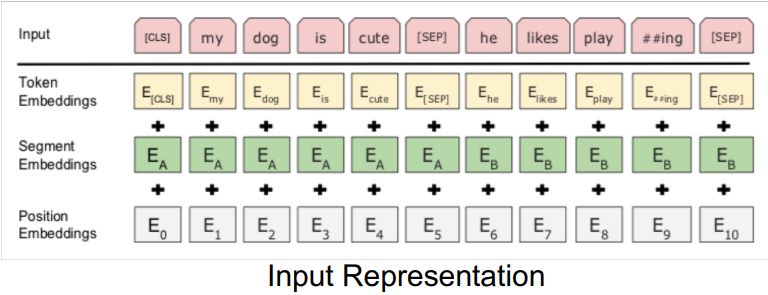
\includegraphics[scale=0.9]{example.png}
	\caption{在此填写图片的标题}
\end{figure}



插入表格:
\begin{tabular}{|c|c|}% 通过添加 | 来表示是否需要绘制竖线
\hline  % 在表格最上方绘制横线
(1,1)&(1,2)\\
\hline  %在第一行和第二行之间绘制横线
(2,1)&(2,2)\\
\hline % 在表格最下方绘制横线
\end{tabular}

\subsection{小节}

在此填写小节内容

\subsubsection{小小节}

在此填写小小节内容

\

\section{结论}

在此填写结论

\

\

\section*{参考文献}

在此填写参考文献
\end{CJK}
\end{document}